\documentclass[border=1pt]{standalone}
% ---------------------------------------------------------------------------
% Shared style for the MOSAIC / CRYSTAL TOMM figures.
% Compile each fig_*.tex with LuaLaTeX (standalone). Sized for acmart
% "acmsmall" (TOMM): \textwidth = 13.9 cm, so every figure is drawn at
% final size and is included with width=\textwidth (no rescaling of text).
% Fonts: Libertinus Sans + Inconsolata (acmart uses Libertine + Inconsolata).
% ---------------------------------------------------------------------------
\usepackage{fontspec}
\setmainfont{LibertinusSans}[Path=fonts/, Extension=.otf,
  UprightFont=*-Regular, BoldFont=*-Bold, ItalicFont=*-Italic]
\setmonofont{Inconsolata}[Path=fonts/, Extension=.otf,
  UprightFont=*-Regular, BoldFont=*-Bold, Scale=0.98]
\usepackage{unicode-math}
\setmathfont{LibertinusMath-Regular.otf}[Path=fonts/]

\usepackage{tikz}
\usetikzlibrary{positioning,fit,calc,arrows.meta,backgrounds,
  shapes.misc,shapes.geometric,decorations.pathreplacing,patterns.meta}

% Okabe-Ito palette (colour-blind safe) + tints -------------------------------
\definecolor{oiBlue}{HTML}{0072B2}
\definecolor{oiOrange}{HTML}{E69F00}
\definecolor{oiSky}{HTML}{56B4E9}
\definecolor{oiGreen}{HTML}{009E73}
\definecolor{oiVerm}{HTML}{D55E00}
\definecolor{oiPurple}{HTML}{CC79A7}
\definecolor{oiYellow}{HTML}{F0E442}
\definecolor{ink}{HTML}{1A1A1A}
\definecolor{muted}{HTML}{5C5C5C}
\definecolor{rule}{HTML}{9A9A9A}

\definecolor{oursFill}{HTML}{DDEBF7}
\definecolor{oursDraw}{HTML}{0072B2}
\definecolor{modFill}{HTML}{FCEFD2}
\definecolor{modDraw}{HTML}{B57600}
\definecolor{upFill}{HTML}{F1F1F1}
\definecolor{upDraw}{HTML}{7D7D7D}
\definecolor{failFill}{HTML}{FBE3D6}
\definecolor{okFill}{HTML}{D9F0E8}

% Sequence colours (as in the packetization study)
\definecolor{seqSOL}{HTML}{0072B2}
\definecolor{seqTHA}{HTML}{009E73}
\definecolor{seqLON}{HTML}{CC79A7}

% Typography -----------------------------------------------------------------
\newcommand{\figfont}{\fontsize{7.5}{9}\selectfont}
\newcommand{\smallfig}{\fontsize{6.5}{7.8}\selectfont}
\newcommand{\tinyfig}{\fontsize{6}{7.2}\selectfont}
\newcommand{\code}[1]{{\ttfamily #1}}

% Provenance encoding: colour AND line style (grayscale safe) ------------------
%  ours      = new component written by us      (blue, solid 0.9 pt)
%  modified  = upstream component we patched    (orange, dashed 0.8 pt)
%  upstream  = used unmodified / third party    (grey, solid 0.45 pt)
\tikzset{
  base/.style={rectangle, rounded corners=1.6pt, align=center,
    inner xsep=3pt, inner ysep=2.6pt, font=\figfont, text=ink,
    execute at begin node={\hyphenpenalty=10000\exhyphenpenalty=10000}},
  ours/.style={base, fill=oursFill, draw=oursDraw, line width=0.9pt},
  mod/.style={base, fill=modFill, draw=modDraw, line width=0.8pt,
    dash pattern=on 2.6pt off 1.4pt},
  up/.style={base, fill=upFill, draw=upDraw, line width=0.45pt},
  dead/.style={base, fill=white, draw=oiVerm, line width=0.6pt,
    dash pattern=on 1.2pt off 1.2pt, text=oiVerm},
  note/.style={font=\smallfig, text=muted, align=left,
    execute at begin node={\hyphenpenalty=10000\exhyphenpenalty=10000}},
  lab/.style={font=\smallfig\itshape, text=muted},
  zone/.style={draw=rule, line width=0.45pt, rounded corners=3pt,
    dash pattern=on 0.6pt off 1.1pt},
  zonetitle/.style={font=\figfont\bfseries, text=ink, anchor=west,
    inner xsep=2pt, inner ysep=1pt, fill=white, xshift=2.5mm},
  flow/.style={-{Stealth[length=4pt,width=3.2pt]}, line width=0.65pt,
    draw=ink},
  dflow/.style={flow, dash pattern=on 2pt off 1.4pt},
  ctrl/.style={-{Stealth[length=3.4pt,width=2.8pt]}, line width=0.5pt,
    draw=muted},
  failflow/.style={-{Stealth[length=4pt,width=3.2pt]}, line width=0.6pt,
    draw=oiVerm, dash pattern=on 1.4pt off 1.2pt},
  stepc/.style={circle, fill=ink, text=white, inner sep=0pt,
    minimum size=8.5pt, font=\tinyfig\bfseries},
  tag/.style={font=\tinyfig\bfseries, inner sep=1pt},
}

% Legend for the provenance encoding -------------------------------------------
\newcommand{\provlegend}[1]{% #1 = anchor coordinate (north west)
  \begin{scope}[shift={(#1)}]
    \node[ours, minimum width=6mm, minimum height=2.6mm, inner sep=0pt]
      (lg1) at (0,0) {};
    \node[anchor=west, font=\smallfig] at (lg1.east) {new (this work)};
    \node[mod, minimum width=6mm, minimum height=2.6mm, inner sep=0pt]
      (lg2) at (2.6,0) {};
    \node[anchor=west, font=\smallfig] at (lg2.east) {upstream, patched by us};
    \node[up, minimum width=6mm, minimum height=2.6mm, inner sep=0pt]
      (lg3) at (6.2,0) {};
    \node[anchor=west, font=\smallfig] at (lg3.east) {upstream / third party, unmodified};
  \end{scope}}

\newcommand{\bx}[2]{{\bfseries #1\par}\vspace{0.6pt}{\smallfig #2\par}}
\begin{document}
\figfont
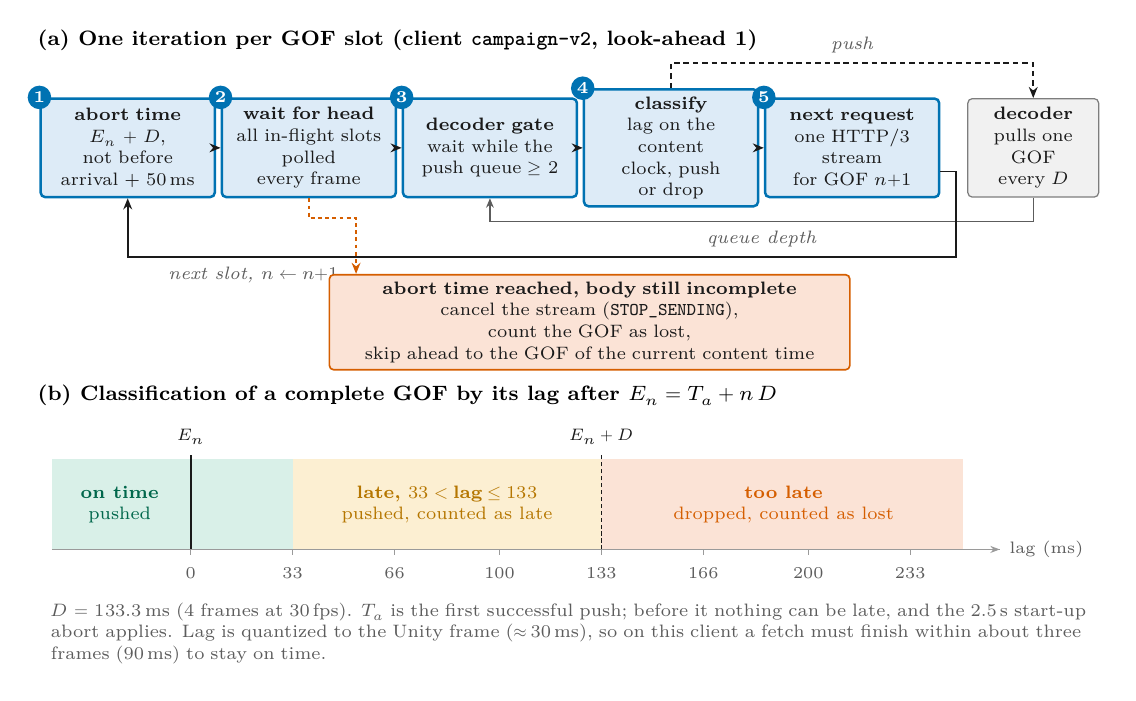
\begin{tikzpicture}[x=1cm,y=1cm]
  \tikzset{panel/.style={font=\figfont\bfseries, anchor=north west, inner sep=0pt},
           st/.style={ours, text width=2.0cm, minimum height=1.25cm, font=\smallfig},
           num/.style={stepc, fill=oiBlue}}

  % ======================= (a) per-slot loop ==================================
  \node[panel] at (0,6.35) {(a) One iteration per GOF slot (client \code{campaign-v2}, look-ahead 1)};

  \node[st] (s1) at (1.15,4.85) {\textbf{abort time}\\$E_n + D$, not before\\arrival + 50\,ms};
  \node[st] (s2) at (3.45,4.85) {\textbf{wait for head}\\all in-flight slots\\polled every frame};
  \node[st] (s3) at (5.75,4.85) {\textbf{decoder gate}\\wait while the\\push queue $\geq 2$};
  \node[st] (s4) at (8.05,4.85) {\textbf{classify}\\lag on the content\\clock, push or drop};
  \node[st] (s5) at (10.35,4.85) {\textbf{next request}\\one HTTP/3 stream\\for GOF $n{+}1$};
  \node[up, text width=1.45cm, minimum height=1.25cm, font=\smallfig] (dec) at (12.65,4.85)
    {\textbf{decoder}\\pulls one GOF\\every $D$};
  \foreach \i in {1,...,5}{ \node[num] at (s\i.north west) {\i}; }
  \draw[flow] (s1) -- (s2); \draw[flow] (s2) -- (s3); \draw[flow] (s3) -- (s4);
  \draw[flow] (s4) -- (s5);
  \draw[dflow] (s4.north) -- ++(0,0.32) -| (dec.north) node[pos=0.25, above, lab] {push};
  \draw[ctrl] (dec.south) -- ++(0,-0.3) -| (s3.south) node[pos=0.25, below, lab] {queue depth};
  \draw[flow] (s5.east) ++(0,-0.3) -- ++(0.2,0) |- ($(s1.south)+(0,-0.75)$) -- (s1.south);
  \node[lab, anchor=north] at ($(s1.south)+(1.6,-0.75)$) {next slot, $n \leftarrow n{+}1$};
  % timeout branch
  \node[base, fill=failFill, draw=oiVerm, line width=0.6pt, font=\smallfig,
        text width=6.4cm, anchor=north west] (to) at (3.7,3.25)
    {\textbf{abort time reached, body still incomplete}\\cancel the stream (\code{STOP\_SENDING}), count the GOF as lost,\\skip ahead to the GOF of the current content time};
  \draw[failflow] (s2.south) -- ++(0,-0.25) -| ($(to.north west)+(0.35,0)$);

  % ======================= (b) lag classification =============================
  \node[panel] at (0,1.85) {(b) Classification of a complete GOF by its lag after $E_n = T_a + n\,D$};
  % axis: x = 0.75 + lag/30 (cm); range -45 .. 260 ms
  \def\X#1{(1.95+#1/25.5)}
  \begin{scope}[yshift=-0.85cm]
    \fill[okFill]   ({1.95+(-45)/25.5},0.6) rectangle ({1.95+33/25.5},1.75);
    \fill[modFill]  ({1.95+33/25.5},0.6) rectangle ({1.95+133/25.5},1.75);
    \fill[failFill] ({1.95+133/25.5},0.6) rectangle ({1.95+250/25.5},1.75);
    \draw[rule, line width=0.45pt] ({1.95+(-45)/25.5},0.6) -- ({1.95+262/25.5},0.6);
    \draw[-{Stealth[length=3.4pt]}, rule, line width=0.45pt] ({1.95+250/25.5},0.6) -- ({1.95+262/25.5},0.6);
    \foreach \t in {0,33,66,100,133,166,200,233}{
      \draw[rule, line width=0.4pt] ({1.95+\t/25.5},0.6) -- ++(0,-0.07);
      \node[font=\tinyfig, anchor=north, text=muted] at ({1.95+\t/25.5},0.5) {\t};}
    \node[font=\tinyfig, anchor=west, text=muted] at ({1.95+262/25.5},0.6) {lag (ms)};
    \draw[ink, line width=0.6pt] ({1.95+0/25.5},0.6) -- ({1.95+0/25.5},1.8) node[above, font=\tinyfig] {$E_n$};
    \draw[ink, line width=0.6pt, dash pattern=on 1.5pt off 1pt] ({1.95+133/25.5},0.6) -- ({1.95+133/25.5},1.8)
       node[above, font=\tinyfig] {$E_n + D$};
    \node[font=\smallfig, align=center, text=oiGreen!65!black] at ({1.95+(-23)/25.5},1.17)
       {\textbf{on time}\\pushed};
    \node[font=\smallfig, align=center, text=modDraw] at ({1.95+83/25.5},1.17)
       {\textbf{late, $33 < \text{lag} \leq 133$}\\pushed, counted as late};
    \node[font=\smallfig, align=center, text=oiVerm] at ({1.95+192/25.5},1.17)
       {\textbf{too late}\\dropped, counted as lost};
    \node[note, anchor=north west, text width=13.3cm] at (0.05,0.05)
      {$D = 133.3$\,ms (4 frames at 30\,fps). $T_a$ is the first successful push; before it nothing can be late, and the 2.5\,s start-up abort applies. Lag is quantized to the Unity frame ($\approx$\,30\,ms), so on this client a fetch must finish within about three frames (90\,ms) to stay on time.};
  \end{scope}
\end{tikzpicture}
\end{document}
